% Final report, ACL format. Build: pdflatex report && bibtex report && pdflatex report && pdflatex report
\documentclass[11pt]{article}
\usepackage[final]{acl}
\usepackage{times}
\usepackage{latexsym}
\usepackage[T1]{fontenc}
\usepackage[utf8]{inputenc}
\usepackage{microtype}
\usepackage{amsmath,amssymb}
\usepackage{booktabs}
\usepackage{tabularx}
\usepackage{multirow}
\usepackage{enumitem}
\usepackage{placeins}
\usepackage{tikz}
\usetikzlibrary{positioning,fit,backgrounds,arrows.meta}
\setlist{topsep=2pt,itemsep=1pt,parsep=0pt,leftmargin=*}
\newcommand{\tool}[1]{\texttt{\small #1}}
\newcommand{\ra}{$\rightarrow$}
\newcolumntype{Y}{>{\raggedright\arraybackslash}X}

\title{Correction Inception: A Small Open VLM Detects, but Cannot Yet Correct,\\Grade-Changing Transcription Errors in Handwritten Exams}

\author{Prabhav \\ 2023115008 \And Jayanth \\ 2023115016 \And Saloni \\ 2023115001 \And Sampath \\ 2023102033 \AND
  Team Dropouts, LMA Group Project 2026 \\
  \texttt{\url{https://github.com/TOMATOsJr/Correction-Inception}}}

\renewcommand{\topfraction}{0.9}\renewcommand{\dbltopfraction}{0.9}\renewcommand{\textfraction}{0.07}\setcounter{topnumber}{4}\setcounter{dbltopnumber}{3}
\begin{document}
\maketitle

\begin{abstract}
AI grading of handwritten work usually runs in two steps: a vision-language model (VLM) transcribes the page, and a language model grades the transcript. Reading mistakes become grading mistakes in two directions. A \emph{misread} costs the student marks they earned; a \emph{silent correction} (``correction inception'') happens when the reader quietly fixes the student's mistake, giving marks the student did not earn. We rebuilt the evaluation of EDU-CIRCUIT-HW and added a grade-impact metric, the \emph{transcription-caused grading error} (TCE): the share of rubric codes whose deduction changes when the same grader reads the AI transcript instead of the expert one. TCE is 8.1\% for Gemini 2.5 Pro and 28.6\% for our reader. Our main finding is that a small open model, Qwen2.5-VL-3B, is good enough to \textbf{detect} these errors but not to \textbf{correct} them. Fine-tuned with QLoRA, it transcribes almost verbatim (token error 34.9\%\ra8.5\% on FERMAT; answers silently corrected 22.2\%\ra14.0\%), and its own confidence detects misreads with AUROC 0.75 on its transcripts and 0.83 on Gemini's, while a blank-image test detects silent corrections with AUROC 0.92. Deciding what the flagged number really is lies beyond it: as a fine-tuned A/B checker it keeps 99.5\% of correct numbers but picks the true value of a misread only 57\% of the time. So the best automatic correction is net $+2$ of 304 misreads, tool-calling Advocate/Auditor agents do worse than the same tools without agents ($-7$ vs.\ $+1$), although the Auditor halves the Advocate's damage, and verified agents leave TCE unchanged. With this model the system is a reliable detector and triage tool, not yet an automatic corrector.
\end{abstract}

% ======================================================================
\section{Introduction}

Recent work shows that even frontier VLMs misread a large share of handwritten university answers, with sample error rates from 38\% to 86\% \citep{educircuit2026}. When a grader uses these transcripts, a wrong digit can cost a student marks for work they did correctly. Silent corrections are harder to spot, because the transcript then looks \emph{better} than what the student wrote.

Our goal is fairer grades, not a better OCR, and the system should be automatic, so that a teaching assistant (TA) only sees what the system cannot resolve. We ask four questions:
\begin{enumerate}
  \item How much grading error is caused by transcription alone, and in which direction?
  \item Can a small reader be fine-tuned to transcribe \emph{verbatim}, i.e.\ not silently correct?
  \item Can the errors that matter be detected from the reader's own uncertainty?
  \item Can two opposing agents fix them under strict verification, and beat the same tools used without agents? The \textbf{Advocate} argues for the student (misreads); the \textbf{Auditor} argues against unearned marks (silent corrections). Verification uses what is written (a context-free re-read, a forced choice, the student's own work), never mathematical correctness.
\end{enumerate}

\paragraph{Main finding.} With a 3B open reader that fits on two 2080 Ti cards (11\,GB each), the answer splits cleanly. Detection works: the reader knows \emph{where} it is unsure, and a page-free re-score shows \emph{where} it guessed from context. Correction does not: knowing where it is unsure does not tell the model \emph{what} is written, and every tool or agent built on its judgement stays within noise. We therefore present the system as a detector whose output is reliable, and report the correction layer as a negative result with its cause.

\paragraph{Contributions.}
\begin{itemize}
  \item A model-agnostic re-implementation of the EDU-CIRCUIT-HW evaluation that recomputes the paper's range of sample error rates (37.6--85.6\% vs.\ 37.62--85.43\%).
  \item TCE, a grade-impact metric with student-clustered bootstrap CIs (the paper's version is unreleased).
  \item A verbatim reader (QLoRA on FERMAT) and an exact silent-correction metric.
  \item \textbf{Detection} of both error types: misreads by teacher-forced token confidence, usable on any transcript including closed-model ones, plus a learned selector; silent corrections by a blank-image signal.
  \item Correction tools measured one by one against expert transcripts: forced-choice A/B verification, a fine-tuned checker, digit beam candidates, blank-image and answer-key guards, page consistency and a learned Arbiter.
  \item Two generations of Advocate/Auditor agents, a full ablation study, and a comparison against the same tools without agents.
\end{itemize}

% ======================================================================
\section{Literature Review}

\paragraph{Handwritten STEM recognition and grading.} EDU-CIRCUIT-HW \citep{educircuit2026} provides expert-rectified transcripts, TA rubric grades and a judge-based error metric (SER/AEC) with a four-way taxonomy. We reuse its prompts and its released transcripts from six VLMs. The paper discusses but does not release a grade-impact measurement.

\paragraph{Over-correction by VLMs.} FERMAT \citep{fermat2025} contains handwritten maths answers with planted errors (\tool{pert\_a} as written, \tool{orig\_a} correct) and shows that VLMs often ``fix'' student errors while transcribing, which is exactly our silent-correction failure.

\paragraph{Parameter-efficient fine-tuning.} We use LoRA \citep{hu2022lora} and QLoRA \citep{dettmers2023qlora} on Qwen2.5-VL-3B-Instruct \citep{qwen25vl}, for both the reader and the A/B checker; agents and the grader use Qwen2.5-7B-Instruct \citep{qwen25}.

\paragraph{Self-correction, verification and debate.} Asking an LLM to revise its own output (our baseline B2) is unreliable without external feedback \citep{huang2024selfcorrect}. Debate-style setups route claims through opposing agents \citep{irving2018debate,du2024debate}. We keep the debate idea, but a rule-based or learned Arbiter decides from tool evidence, not an LLM.

\paragraph{Uncertainty and tool use.} Token-level confidence is a standard signal for OCR and generation errors; we compute it by teacher forcing, so it also works for transcripts without released logits. Our second agent generation calls tools in a structured format \citep{schick2023toolformer}, so that claims rest on evidence rather than on the agent's own reading.

\paragraph{LLM-as-judge.} Judge reliability varies \citep{zheng2023judge}. Our free Qwen-7B judge agreed with Gemini almost not at all ($\kappa=0.03$), so we replaced it with an exact maths-token comparison.

% ======================================================================
\section{Datasets}

We use two public datasets, summarised in Table~\ref{tab:data}.

\begin{table}[h]
\centering\small
\begin{tabularx}{\columnwidth}{@{}lY@{}}
\toprule
& \textbf{EDU-CIRCUIT-HW} \\
Size & 1,334 answers; observation set 513 answers, 11 students, TA marks per rubric code; 293 with expert transcripts; 62 rubrics \\
Truth & expert transcripts, TA grades, rubrics, 6 released VLM transcripts, judge verdicts \\
Use & main evaluation (TCE, maths diff, misread labels) \\
\midrule
& \textbf{FERMAT} \\
Size & 2,244 answers; problem-level split 1,567 train / 425 test (360 usable for silent correction) \\
Truth & \tool{pert\_a} (written, with a planted error), \tool{orig\_a} (correct) \\
Use & fine-tuning the reader and the checker; exact silent-correction labels \\
\bottomrule
\end{tabularx}
\caption{Datasets used.}
\label{tab:data}
\end{table}

On top of these two datasets we created:
\begin{itemize}
  \item \textbf{Per-number misread labels}, aligning every transcript number to the expert transcript: 7,701 numbers with 680 misreads (8.8\%) for our reader; 10,310 numbers with 116 misreads (1.1\%) for Gemini 2.5 Pro.
  \item \textbf{Per-number FERMAT labels} (ok / misread / silent) for our reader's test outputs: 8,916 numbers, 57 misreads, 18 silent corrections.
  \item \textbf{A/B checker training pairs} of three kinds, balanced per source and kind: silent (FERMAT), look-alike digit swaps (3$\leftrightarrow$8, 1$\leftrightarrow$7, \dots), and EDU near-miss misreads from 3 students, who are excluded from every evaluation.
  \item \textbf{An 80-exam ablation subset}.
\end{itemize}
The expert transcripts are corrected Gemini 2.5 Pro output, which favours Gemini 2.5. We never called the commercial APIs; their transcripts came with the dataset. Student data (transcripts, per-number label and score files, agent ledgers) is never committed.

% ======================================================================
\section{Methodology}

\begin{figure*}[t]
\centering
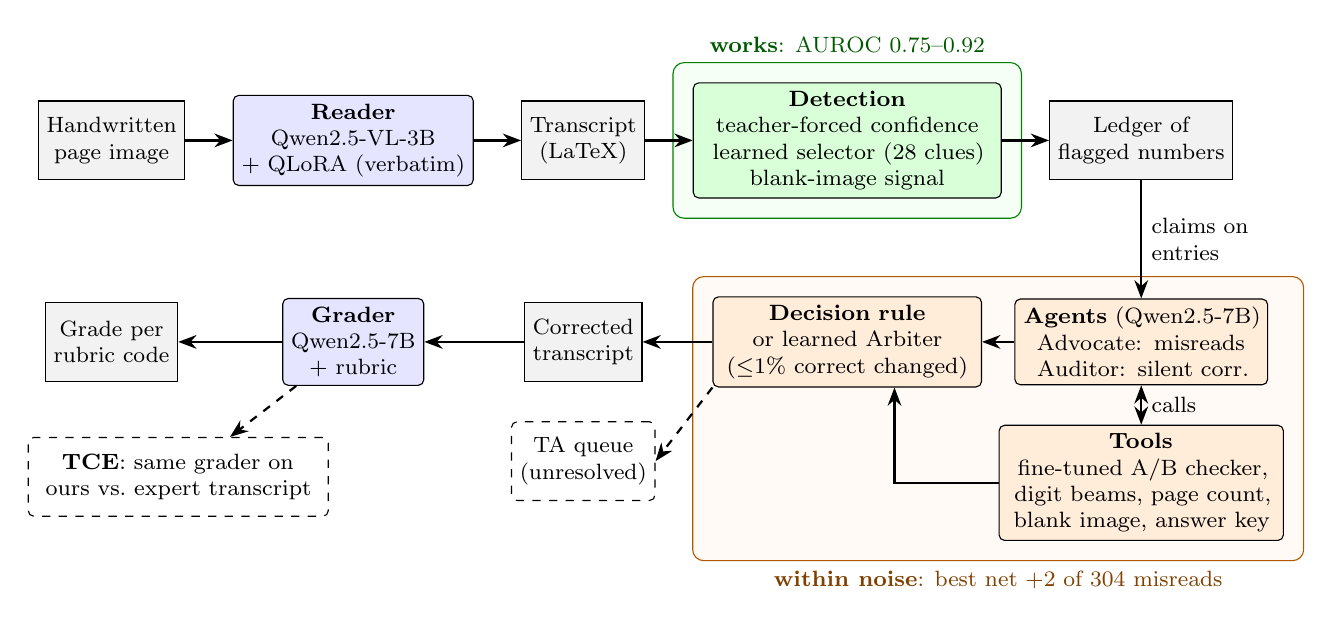
\begin{tikzpicture}[font=\footnotesize, >=Stealth, node distance=5mm and 6mm,
  box/.style={draw, rounded corners=2pt, align=center, inner sep=3pt, minimum height=10mm},
  data/.style={box, fill=gray!10, rounded corners=0pt},
  model/.style={box, fill=blue!10},
  det/.style={box, fill=green!15},
  cor/.style={box, fill=orange!15},
  arr/.style={->, thick}]
% row 1: reading and detection
\node[data] (page) {Handwritten\\page image};
\node[model, right=of page] (reader) {\textbf{Reader}\\Qwen2.5-VL-3B\\+ QLoRA (verbatim)};
\node[data, right=of reader] (tr) {Transcript\\(LaTeX)};
\node[det, right=of tr, text width=3.7cm] (detect) {\textbf{Detection}\\teacher-forced confidence\\learned selector (28 clues)\\blank-image signal};
\node[data, right=of detect] (ledger) {Ledger of\\flagged numbers};
% row 2: correction and grading (right to left)
\node[cor, below=15mm of ledger, text width=3.0cm] (agents) {\textbf{Agents} (Qwen2.5-7B)\\Advocate: misreads\\Auditor: silent corr.};
\node[cor, text width=3.2cm] (rule) at (detect |- agents) {\textbf{Decision rule}\\or learned Arbiter\\($\leq$1\% correct changed)};
\node[data] (fixed) at (tr |- agents) {Corrected\\transcript};
\node[model] (grader) at (reader |- agents) {\textbf{Grader}\\Qwen2.5-7B\\+ rubric};
\node[data] (grade) at (page |- agents) {Grade per\\rubric code};
% row 3: tools, TA queue, evaluation
\node[cor, below=5mm of agents, text width=3.4cm] (tools) {\textbf{Tools}\\fine-tuned A/B checker,\\digit beams, page count,\\blank image, answer key};
\node[box, dashed, below=5mm of fixed] (ta) {TA queue\\(unresolved)};
\node[box, dashed, below=7mm of grade.south east, anchor=north, text width=3.6cm] (tce) {\textbf{TCE}: same grader on\\ours vs.\ expert transcript};
% arrows
\draw[arr] (page) -- (reader);
\draw[arr] (reader) -- (tr);
\draw[arr] (tr) -- (detect);
\draw[arr] (detect) -- (ledger);
\draw[arr] (ledger) -- node[right, align=left]{claims on\\entries} (agents);
\draw[<->, thick] (agents) -- node[right]{calls} (tools);
\draw[arr] (agents) -- (rule);
\draw[arr] (tools.west) -| ([xshift=6mm]rule.south);
\draw[arr] (rule) -- (fixed);
\draw[arr, dashed] (rule.south west) -- (ta.east);
\draw[arr] (fixed) -- (grader);
\draw[arr] (grader) -- (grade);
\draw[arr, dashed] (grader) -- (tce);
% stage bands
\begin{scope}[on background layer]
\node[draw=green!50!black, fill=green!4, rounded corners, inner sep=2.5mm, fit=(detect), label={[green!35!black]above:\textbf{works}: AUROC 0.75--0.92}] {};
\node[draw=orange!70!black, fill=orange!4, rounded corners, inner sep=2.5mm, fit=(agents)(rule)(tools), label={[orange!50!black]below:\textbf{within noise}: best net $+2$ of 304 misreads}] {};
\end{scope}
\end{tikzpicture}
\caption{Architecture. The fine-tuned 3B reader transcribes the page; detection flags numbers that may be misread or silently corrected (green, reliable). The correction layer (orange) lets the Advocate and the Auditor argue over each flagged number with tool evidence, and a fixed rule or learned Arbiter decides; anything it cannot settle goes to a TA. TCE compares the grade from our transcript with the grade from the expert transcript.}
\label{fig:arch}
\end{figure*}

Figure~\ref{fig:arch} shows the whole system.

\subsection{Evaluation pipeline}
\tool{run\_ocr.py} transcribes pages with any backend; \tool{evaluate\_recognition.py} reproduces the paper's judge, filter, SER/AEC and taxonomy steps; \tool{transcript\_diff.py} compares numbers, operators and variables inside LaTeX maths with the expert transcript. \tool{grade\_impact.py} computes \textbf{TCE}: the same grader (Qwen2.5-7B-Instruct, 4-bit) marks the expert and the AI transcript against the rubric, and every (answer, rubric code) pair whose deduction differs is an error, split into wrongful deduction and over-credit, with student-clustered bootstrap CIs. The grader agrees with TAs 71\% of the time; its noise floor is 6.7\%.

\subsection{Verbatim reader}
We fine-tuned Qwen2.5-VL-3B-Instruct with QLoRA on FERMAT to reproduce \tool{pert\_a} (what is written) rather than \tool{orig\_a}. FERMAT marks the planted error with \verb|\textcolor{red}{...}|; we strip these markers from the training target and from all metrics. The \emph{silent-correction rate} asks whether, at the spots where \tool{pert\_a} and \tool{orig\_a} differ, the output matches the correct version better than the written one.

\subsection{Misread detection}
\textbf{Teacher-forced confidence:} the transcript under test is fed in as the reader's answer, and one forward pass gives each number's negative log-likelihood, digit entropy, probability gap and the reader's preferred alternative digits. \textbf{Learned selector:} a logistic regression over 28 clues (own doubt, page doubt, rank on the page, neighbours, digit shape, look-alikes), cross-validated in folds split by student. \textbf{Blank-image signal (Auditor):} the transcript is scored again with a white image; a number predicted just as well without the page comes from context, not from the ink, which is the signature of a silent correction.

\subsection{Correction tools}
\textbf{Candidates} come from appearance only, never from the answer key: the reader's alternative digits, look-alike swaps, and a digit-by-digit \textbf{beam search} that reads the page once and then searches on the cached keys and values, so it fits on a 2080 Ti (11\,GB). The \textbf{forced choice} asks the reader ``Is the number marked [?] written as A) $x$ or B) $y$?'' in both option orders, reading the answer-letter logits. The \textbf{fine-tuned A/B checker} trains the reader's LoRA further on the pairs, with the loss on the answer letter only; \tool{checker\_f} uses FERMAT only and \tool{checker\_fe} adds the 3 EDU students. A change is blocked if the candidate equals the rubric's expected value (\textbf{answer-key guard}) or if the checker prefers it almost as much on a blank image (\textbf{blank-image guard}). The \textbf{decision rule} changes a number only if both orders agree and the change probability $\geq\tau$, with $\tau$ set on the other students so that at most 1\% of their correct numbers change. Alternatives: a \textbf{learned Arbiter} (one logistic model over all evidence, trained on other students) and \textbf{page consistency} (does the candidate, or the written value, appear elsewhere on the page?).

\subsection{Agents}
\paragraph{Generation 1: free-text claims.} The Advocate and the Auditor (Qwen2.5-7B-Instruct) file claims that quote a span and change one number. Tools are \tool{crop\_reread} (a context-free re-read by the fine-tuned reader with the disputed value masked) and consistency with the student's later lines. In the \emph{one-shot} protocol agents file claims, tools run and the Arbiter decides; in the \emph{interactive} protocol (r1, tools, r2, tools, r3) agents may counter, withdraw, revise or concede. The rule-based Arbiter ($\theta=0.85$) accepts a claim only with supporting evidence, rejects contradicted ones and escalates the rest to a TA.

\paragraph{Generation 2: tool-calling agents over a ledger.} Generation~1 failed mainly because its claims could not be verified (\S\ref{sec:eval}), so generation~2 fixes the claim format. Agents see a numbered ledger of the page's flagged numbers; a claim names one entry and one candidate, so every claim is checkable. Tools are \tool{checker}, \tool{beams}, \tool{page\_count}, \tool{blank} and \tool{answer\_key} (up to 8 calls per round, 2 rounds per agent). The Advocate files claims, the Auditor objects to unsupported ones, and a fixed rule applies the survivors.

\subsection{Baselines}
\textbf{B1}: no correction. \textbf{B2}: one-pass LLM self-correction. \textbf{No-verify}: every agent claim applied unchecked. \textbf{Pipeline}: the same tools and rule without agents, which the agents must beat.

% ======================================================================
\section{Experiment Runs}

\begin{table*}[t]
\centering\small
\begin{tabularx}{\textwidth}{@{}lllY@{}}
\toprule
Run & Where & Branch & What \\
\midrule
Paper reproduction & CPU & \tool{main} & SER/AEC for 6 VLMs from released verdicts \\
Kaggle runs 1--2 & Kaggle T4 & \tool{main} & TCE of released transcripts; judge calibration \\
PC run & RTX 5070 Ti & \tool{main} & our reader (untuned and QLoRA); FERMAT eval \\
Agent full run & 2$\times$2080 Ti (11\,GB) & \tool{agent\_interaction} & 214 exams, interactive agents, 5 variants \\
Colab runs & Colab & \tool{colab-results} & 50-exam agent run; misread detection \\
Misread detection & 2$\times$2080 Ti (11\,GB) & \tool{misread\_detection} & confidence AUROC per transcriber and reader \\
Correction & 2$\times$2080 Ti (11\,GB) & \tool{forced\_choice} & selector, forced choice, guards; held-out students \\
A/B checker & 2$\times$2080 Ti (11\,GB) & \tool{ab\_checker} & checker training and eval; correction at 3/10/20 numbers per page; Arbiter; consistency; Auditor on FERMAT and EDU; tool-calling agents \\
Ablation & 2$\times$2080 Ti (11\,GB), 3h23m & \tool{ablation-results} & 80 exams $\times$ 2 transcribers; ablations \#2, \#3, \#6, \#7, \#9, \#10, \#16 \\
\bottomrule
\end{tabularx}
\caption{Experiment runs and the repository branch that holds each.}
\label{tab:runs}
\end{table*}

Table~\ref{tab:runs} lists all runs.

\subsection{Measurement}

\begin{table}[t]
\centering\small
\begin{tabular}{@{}lccc@{}}
\toprule
Transcriber & SER & 95\% CI & AEC \\
\midrule
Gemini 3 Pro & 37.6 & 31.7--42.9 & 0.62 \\
Gemini 2.5 Pro & 53.4 & 48.0--59.9 & 1.23 \\
Qwen3-VL-Plus & 61.8 & 53.5--69.7 & 1.38 \\
GPT-5.1 & 71.5 & 62.8--79.5 & 2.05 \\
Claude Sonnet 4.5 & 80.7 & 74.4--87.1 & 2.77 \\
Qwen3-VL-8B (thinking) & 85.6 & 79.7--91.5 & 2.81 \\
\bottomrule
\end{tabular}
\caption{Recognition with the paper's method (513 samples). SER in \%.}
\label{tab:ser}
\end{table}

\begin{table}[t]
\centering\footnotesize
\setlength{\tabcolsep}{3pt}
\begin{tabular}{@{}lccccc@{}}
\toprule
Transcriber & TCE & Wr. & Over & Ex.\ aff. & Ex.\ num. \\
\midrule
Gemini 2.5 Pro & 8.1 & 5.5 & 2.6 & 25 & 45 \\
Gemini 3 Pro & 16.4 & 9.9 & 6.5 & 45 & 74 \\
GPT-5.1 & 18.0 & 12.0 & 6.0 & 51 & 83 \\
Qwen-3B base & 32.9 & 27.8 & 5.1 & 73 & 95.6 \\
Qwen-3B QLoRA & \textbf{28.6} & 22.8 & 5.8 & 71 & 91.8 \\
\bottomrule
\end{tabular}
\caption{Grade impact (\%), Qwen-7B grader; Qwen-3B QLoRA is our reader. Wr.: wrongful deduction; Over: over-credit; Ex.\ aff.: exams with a changed grade; Ex.\ num.: exams with any wrong number.}
\label{tab:tce}
\end{table}

Tables~\ref{tab:ser} and~\ref{tab:tce} show that recognition rank does not predict grade damage: Gemini 3 has the best SER but twice the TCE of Gemini 2.5 (partly because the answer key also derives from Gemini 2.5). With the paper's own grader against TA grades, grading disagreement is 59.1\% on answers with recognition errors vs.\ 36.8\% without.

\subsection{Fine-tuning}

\begin{table}[t]
\centering\footnotesize
\setlength{\tabcolsep}{3pt}
\begin{tabular}{@{}lccc@{}}
\toprule
Reader & Ans.\ silent & Spots silent & Token err. \\
\midrule
Qwen2.5-VL-3B base & 22.2 & 8.8 & 34.9 \\
+ our QLoRA & \textbf{14.0} & \textbf{4.9} & \textbf{8.5} \\
\bottomrule
\end{tabular}
\caption{Verbatim reader on the FERMAT test split, red markers stripped (\%): answers silently corrected, planted-error spots silently corrected, token error against what is written.}
\label{tab:reader}
\end{table}

\begin{table}[t]
\centering\footnotesize
\setlength{\tabcolsep}{3pt}
\begin{tabular}{@{}lcccc@{}}
\toprule
Pairs & Base & Reader & ck\_f & ck\_fe \\
\midrule
EDU misread: picks truth & 53.1 & 51.5 & 46.9 & \textbf{57.1} \\
EDU correct: keeps it & 90.2 & 95.0 & 99.5 & \textbf{99.5} \\
FERMAT wrong: keeps written & 82.2 & 86.9 & \textbf{97.9} & 94.5 \\
FERMAT correct: keeps it & 94.0 & 96.0 & 100 & 99.0 \\
\bottomrule
\end{tabular}
\caption{A/B checker accuracy on held-out pairs (\%), averaged over both option orders; chance is 50\%. $n$ = 196, 400, 382, 400.}
\label{tab:checker}
\end{table}

The reader (Table~\ref{tab:reader}) cuts token errors to about a quarter and silent corrections from 22.2\% to 14.0\% of answers. The checker (Table~\ref{tab:checker}) learned to keep what is written, so it resists silent corrections, but learned only a little about real misreads: \tool{checker\_fe} picks the truth on 57.1\% of EDU misreads, and in both option orders on 49\% (base model: 32\%).

\subsection{Detection}

\begin{table}[t]
\centering\footnotesize
\setlength{\tabcolsep}{3pt}
\begin{tabular}{@{}llc@{}}
\toprule
Signal & Errors to detect & AUROC \\
\midrule
Confidence & misreads, our reader (EDU) & 0.75 \\
Confidence & misreads, Gemini 2.5 (EDU) & 0.83 \\
Blank image & silent corrections (FERMAT) & \textbf{0.92} \\
Digit entropy & silent corrections (FERMAT) & 0.90 \\
\bottomrule
\end{tabular}
\caption{Detection with the fine-tuned 3B reader. EDU: 7,701 (ours) and 10,310 (Gemini) numbers with 680 and 116 misreads; FERMAT: 18 silent corrections vs.\ 8,841 correct numbers. Confidence is teacher-forced.}
\label{tab:detect}
\end{table}

Detection is where the 3B reader is strong (Table~\ref{tab:detect}). Teacher-forced confidence separates misreads with AUROC 0.75 (our reader) and 0.83 (Gemini), so the same small model can audit a closed model's transcript. But the reader's best alternative equals the true number in only 14--28\% of misreads, an early sign that it knows where it is wrong more often than what is right; and about 7\% of misreads get $\geq$99.99\% confidence. At 80\% recall on held-out students, the learned selector flags 44\% of our reader's numbers (29\% of flags real) against 64\% (19\%) for a confidence cut-off; on Gemini, where misreads are rare, it does not help (41\% vs.\ 32\% flagged). For silent corrections on FERMAT, the blank-image signal separates the 18 silent corrections from 8,841 correct numbers with direction-free AUROC \textbf{0.916} (digit entropy: 0.904), and its 4 most suspicious numbers per answer contain 16 of the 18.

\subsection{Correction of EDU misreads}

\begin{table*}[t]
\centering\small
\begin{tabular}{@{}lccccccc@{}}
\toprule
Run & Checked & Truth offered & Fixed & Other wrong & Broken & Net & Misreads \\
\midrule
Untuned reader, forced choice & 845 & -- & 2 & 3 & 7 & $-8$ & -- \\
Reader LoRA, 3 per page & 569 & 34\% & 2 & 1 & 4 & $-3$ & 304\ra306 \\
\tool{checker\_fe}, 3 per page & 569 & 34\% & 5 & 0 & 3 & $\mathbf{+2}$ & 304\ra302 \\
\tool{checker\_fe}, 10 per page + beams & 1,826 & 69\% & 10 & 2 & 7 & $+1$ & 304\ra301 \\
\tool{checker\_fe}, 20 per page + beams & 3,224 & 66\% & 13 & 2 & 11 & $0$ & 304\ra302 \\
\bottomrule
\end{tabular}
\caption{Automatic correction on unseen students (the 3 checker-training students left out; 304 misreads; the first row is the earlier \tool{forced\_choice} run on its own held-out students). Net = fixed $-$ changed to another wrong value $-$ correct numbers broken.}
\label{tab:correct}
\end{table*}

Table~\ref{tab:correct}: beams double the share of misreads whose true value is offered (34\%\ra69\%), but checking more numbers per page breaks as many correct numbers as it fixes. Wrong numbers per exam stay at about 12.96 in every run. With a perfect TA on the \tool{forced\_choice} queue (2.2 numbers per page), misreads would fall from 680 to 517.

% ======================================================================
\section{Ablations}

\begin{table}[t]
\centering\small
\begin{tabular}{@{}lcc@{}}
\toprule
System & qwen3b\_ft & gemini25 \\
\midrule
No correction (B1) & 28.2 & 8.5 \\
B2 self-correction & \textbf{25.0} & \textbf{7.5} \\
One-shot agents + Arbiter & 28.2 & 8.5 \\
Interactive agents + Arbiter & 28.2 & 8.5 \\
Accept every claim & 28.5 & 8.0 \\
Claims accepted (interactive) & 0/112 & 2/123 \\
\bottomrule
\end{tabular}
\caption{80-exam ablation with generation-1 agents: TCE (\%). B1 CIs: 23.0--33.5 and 4.4--13.7; B2 CIs overlap them. Both accepted Gemini claims were harmful.}
\label{tab:ablation}
\end{table}

\paragraph{80-exam ablation (generation 1, Table~\ref{tab:ablation}).}
\textbf{\#9 Headline:} agents leave TCE unchanged; B2 lowers it slightly but adds number errors (mean mismatches 12.5\ra14.7 for our reader, 1.4\ra6.9 for Gemini). \textbf{\#2 Arbiter evidence:} all verified modes give the same TCE; accepting every claim gives claim precision 8.7\% (qwen) and 0\% (gemini), and in the earlier 214-exam run unchecked claims helped 4 times, hurt 64 times and were neutral 394 times (TCE 28.5\ra29.2). \textbf{\#3 Threshold} $\theta\in[0.5,0.95]$: no effect, at most 2 claims accepted. \textbf{\#6/\#7 Re-reader} (base vs.\ fine-tuned, value masked vs.\ shown): resolved re-reads mostly side with the transcribed value, on only 12--32 evaluable claims. \textbf{\#10 Single agent:} Advocate-only and Auditor-only give the same TCE as both. \textbf{\#16 Strong vs.\ weak transcriber:} neither benefits.

\begin{table*}[t]
\centering\small
\begin{tabularx}{\textwidth}{@{}l>{\raggedright\arraybackslash}p{6.2cm}Y@{}}
\toprule
Ablation & Variants (net, of 304 misreads) & Finding \\
\midrule
Checker training data & EDU misreads: base 53.1, reader 51.5, \tool{checker\_f} 46.9, \tool{checker\_fe} \textbf{57.1}\% & EDU near-miss pairs are needed to learn misreads; FERMAT alone teaches ``keep'' \\
Candidate source & true value offered: top-3 digits 34\%; with beams 69\% (10/page), 66\% (20/page) & beams fix the candidate gap, not the choice \\
Numbers per page & 3: \textbf{+2}; 10: +1; 20: 0 & more checks add as many broken numbers as fixes \\
Decision rule & simple +2 / +1 / 0; learned Arbiter, net rule $-9$ to 0; Arbiter, $\leq$1\% budget $-10$ to 0 & the Arbiter ranks better in 3 of 4 runs (AUROC 0.85--0.89 vs.\ 0.81--0.86) but its threshold does not carry over to new students \\
Page consistency & simple +2; veto +2 / +2 / $-13$; \emph{required} (main rule, fixed in advance) $-1$ / $-11$ / $-12$ & the pattern holds for 12.4\% of fixing and 12.6\% of harmful changes: circuit pages reuse the same values \\
\bottomrule
\end{tabularx}
\caption{Checker-side ablations on unseen students. Triples are for 3, 10 and 20 numbers per page.}
\label{tab:ckabl}
\end{table*}

\paragraph{Checker-side ablations (Table~\ref{tab:ckabl}).} None of the decision-rule or candidate variants gets beyond net $+2$.

\begin{table*}[t]
\centering\small
\begin{tabular}{@{}lcccc@{}}
\toprule
Run & Pipeline (no agents) & Advocate + Auditor & Agents as filter only & Advocate alone \\
\midrule
10 per page + beams & $\mathbf{+1}$ (10/2/7) & $-7$ (3/1/9) & $0$ (1/0/1) & $-15$ (6/3/18) \\
20 per page + beams & $\mathbf{0}$ (13/2/11) & $-4$ (1/1/4) & $-2$ (0/1/1) & $-10$ (3/1/12) \\
\bottomrule
\end{tabular}
\caption{Generation-2 tool-calling agents vs.\ the pipeline on 191 pages of unseen students: net (fixed / changed to another wrong value / correct broken).}
\label{tab:agents}
\end{table*}

\paragraph{Generation-2 agents (Table~\ref{tab:agents}).} At 10 numbers per page the Advocate filed 569 claims: only 189 for the value the checker examined, and only 14 would have fixed a misread. The Auditor objected to 368; 164 claims (29\%) failed the format checks. Tool calls were frequent and well formed: 825 checker, 490 beam, 421 page-count, 195 blank-image and 82 answer-key calls, with 8 invalid.

\paragraph{The Auditor on FERMAT.} With the simple rule, the Auditor's fixes change nothing; with the learned Arbiter, silent corrections fall from 18 to 14, plus 2 misreads fixed and 4 correct numbers broken (net $+2$); answers silently corrected go from 13.86\% to 13.55\%.

\paragraph{Silent corrections in real exams.} If our reader silently corrected toward the right answer, misread transcript values would land on answer-key values more often than correctly read numbers do. They do not: 79.1\% of correctly read numbers are key values, but only 56.0\% of misread transcript values (written values: 63.1\%); Gemini shows the same pattern (77.8\%, 42.7\%, 50.4\%). Of our reader's misreads, 89 move toward the key and 137 away from it. The blank-image signal does not carry over: misreads toward the key vs.\ correct numbers score AUROC 0.53, against 0.92 on FERMAT.

\paragraph{Earlier no-API ablations (Gemini 2.5).} An arithmetic-inconsistency flag has 50\% precision; a naive redundancy signal 3.6\%, worse than random (5\%); unit normalisation triples the checkable equalities (45\ra149).

% ======================================================================
\FloatBarrier
\section{Evaluation and Analysis}
\label{sec:eval}

\paragraph{The 3B model is good enough to detect.} Fine-tuning makes the reader faithful: token error falls from 34.9\% to 8.5\% and silent corrections from 22.2\% to 14.0\% of answers, and on EDU, TCE falls from 32.9\% to 28.6\%. On top of it, detection is reliable for both error types: misreads at AUROC 0.75 (own transcripts) and 0.83 (Gemini's), silent corrections at 0.92, with 16 of 18 inside the 4 most suspicious numbers per answer. The fine-tuned checker also almost never changes a correct number (99.5\% kept vs.\ 90.2\%), so the system is safe to run.

\paragraph{The 3B model is not good enough to correct.} Correction needs the model to say \emph{what} a doubtful digit is, and here it is close to chance: the fine-tuned checker picks the true value of an EDU misread 57\% of the time (base model 53\%), and the reader's own best alternative is right in only 14--28\% of misreads. Everything built on this judgement inherits the limit, as the rest of this section shows.

\paragraph{Why generation-1 agents had no effect.} The verifier can only check a claim that changes exactly one number, and most claims changed several numbers or rewrote a line: 83--89 of the 112--123 claims ruled on got no reading, 157 of 203 re-read attempts failed (qwen, interactive), and 653 of 757 failed in the 214-exam run. Without evidence the Arbiter escalates, so transcripts stay unchanged, and the verifier ablations cannot separate the variants.

\paragraph{Generation 2 fixed the format but still loses to the pipeline.} Every claim is now checkable and tools are called correctly, but the agents choose worse than the fixed rule. The Advocate over-claims on numbers and values the checker never examined and drops most changes the pipeline would have made correctly. The Auditor is the useful half: its objections cut the Advocate's damage roughly in half ($-15$\ra$-7$, $-10$\ra$-4$), so adversarial communication helps, but only relative to an unchecked Advocate. As a filter on the pipeline, the agents remove good and bad changes alike.

\paragraph{Why the correction tools are weak.} Detection works (AUROC 0.75--0.83 for misreads, 0.92 for FERMAT silent corrections). Correction is the bottleneck, and it is a model limit rather than a tool limit: the true value is among the candidates for only 34--69\% of misreads, the fine-tuned checker picks it only slightly above chance (57\%), and correct numbers far outnumber misreads among flagged numbers (3,224 checked vs.\ 265 misreads at 20 per page), so every false change cancels a fix. The system follows ``default to keep'': it is safe, but with a 3B reader at capped resolution it is a detector for a TA, not an automatic corrector.

\paragraph{Did the architecture beat no architecture?} The fine-tuned reader and the detection built on it: yes, clearly. The correction layer on top: only within noise (+2 of 304 misreads on EDU, +2 numbers on FERMAT). TCE after correction was not re-measured for the checker runs; a net of 0 to +2 numbers cannot change it measurably given the grader's 6.7\% noise floor.

% ======================================================================
\section{Limitations}
\begin{itemize}
  \item \textbf{Bias in the ground truth.} The expert transcripts are corrected Gemini 2.5 output, and the answer key and grader also lean on it.
  \item \textbf{Small, skewed data.} EDU has 11 students and 293 expert transcripts; Gemini has only 116 misreads; the 3 checker-training students are the messiest, so held-out students are cleaner; FERMAT has only 18 silent corrections for our reader.
  \item \textbf{LLM grader.} Qwen-7B has a 6.7\% noise floor and 71\% TA agreement, so TCE differences of a few points sit inside the CIs. The free judge failed ($\kappa=0.03$) and was replaced by an exact maths diff, which misses non-numeric errors.
  \item \textbf{Scope.} Correction covers numbers only, not variables, operators, dropped lines, diagrams or looping output.
  \item \textbf{Ablation run.} The ``interactive, as built'' row is scored on 55/67 exams, not 80.
  \item \textbf{Compute.} Our main runs use 2$\times$2080 Ti (11\,GB each), which forces a 4-bit grader, a 3B reader and capped image resolution (602,112 pixels). This is the likely cause of the weak correction: the reader cannot resolve the digits it doubts.
  \item \textbf{No human labels.} The planned hand-check of about 100 flags was not done.
\end{itemize}

% ======================================================================
\section{Conclusions}
Transcription alone changes 8--33\% of rubric-level grades, mostly against the student, and recognition rank does not predict grade damage. The Qwen2.5-VL-3B model we could run was good enough for \textbf{detection}: fine-tuned, it reads almost verbatim (token errors cut to about a quarter, silent corrections from 22\% to 14\% of answers), its confidence finds misreads in its own and in Gemini's transcripts (AUROC 0.75 and 0.83), and a blank-image test finds silent corrections (AUROC 0.92). It was not good enough for \textbf{correction}: it picks the true value of a misread barely above chance, so the best verified correction is within noise, the learned Arbiter and page consistency do not help, tool-calling agents lose to the same tools without agents (although the Auditor halves the Advocate's damage), unverified corrections make TCE worse, and only one-pass self-correction lowers TCE, at the cost of new number errors. Detection and correction need different strength: a small model can tell a TA where to look, but deciding what is written needs a stronger reader.

\paragraph{Next steps.} (1) Raise the checker's accuracy on real misreads, the bottleneck: a larger reader, higher-resolution crops, more EDU near-miss data. (2) Train the Advocate's tool-choice policy on the pipeline's outcomes instead of prompting it. (3) Hand-label about 100 flags. (4) Evaluate the system as a TA-triage tool, where it adds value today: a queue of about 2.2 numbers per page that would fix about a quarter of misreads with a TA.

\paragraph{Reproducibility.} Code, run scripts and result summaries: \url{https://github.com/TOMATOsJr/Correction-Inception}. The README on \tool{main} maps every branch and gives one command per experiment.

\bibliography{custom}

\end{document}
